\chapter{Implementierung}

\begin{figure}[ht]
\centering
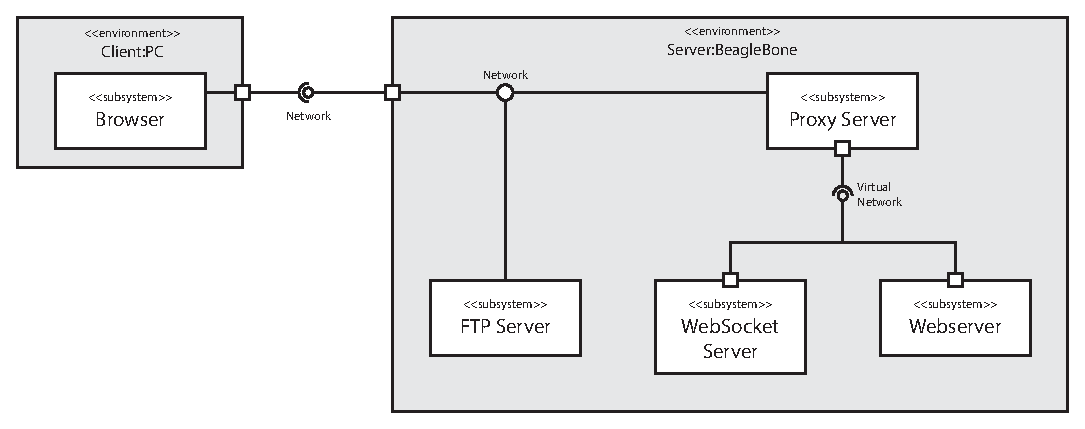
\includegraphics[width = 0.8\textwidth]{images/components.eps}
\caption{Funktionale Komponenten}
\label{fig:functionalComponents}
\end{figure}

Das Webinterface besteht aus drei funktionalen Teilen. Der erste Teil ist der Webbrowser, der ausschließlich als Client dient. Zweitens besteht das Webinterface aus dem WebSocket Server, der die Steuerung der \gls{gpio} erledigt und die Daten für die Konfiguration der Weboberfläche liefert; drittens aus einem Webserver, der die Dokumente ausliefert. Um nach außen über einen einzigen Port zu kommunizieren, ist ein Proxy Server vorgelagert (Abb. \ref{fig:functionalComponents}), der den Datenverkehr an Hand des verwendeten Protokolls an den richtigen Server weiterleitet (Abb. \ref{fig:requestForwarding}).

\begin{figure}[ht]
\centering
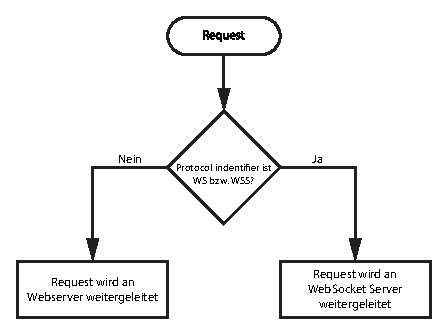
\includegraphics[width = 0.5\textwidth]{images/request.eps}
\caption{Verarbeitungschema eines Requests am Proxy Server}
\label{fig:requestForwarding}
\end{figure}

\noindent Die Auslagerung das Proxy Servers hat folgende Vorteile:

\begin{enumerate}
\item Das \gls{ssl-offloading} wird von HAProxy automatisch vorgenommen.
\item Der Webserver ist nicht direkt zu erreichen. D. h. eventuelle Einbruchsversuche über Fehler in der HTTP-Implemtierung von Lighttpd werden bereits im Proxy Server abgefangen, da ungültige HTTP Header nicht weiterverarbeitet werden.
\item Um die direkte Hardwaresteuerung zu übernehmen, muss der WebSocket Server mit root-Rechten betrieben werden. Da WebSocket Requests nicht durch den Webserver geleitet werden, ist das System selbst bei einer Übernahme des Webservers weitegehend sicher. Zudem ist für den Betrieb keinerlei Kommunikation zwischen Webserver und WebSocket Server notwendig (Vgl. Abb. \ref{fig:pageloadSequence}).
\item Das Projekt gestaltet sich übersichtlicher, da die einzelnen Komponenten über virtuelle Netzwerkverbindungen kommunizieren und somit leichter zu warten sind.   
\item HAProxy ist im Feldeinsatz erprobt und kann angesichts der weiten Verbreitung auf namhaften Webseiten als ausreichend stabil angenommen werden \cite{kuehnast2014}, während die ProxyUnterstützung in Lighttpd nur mäßig dokumentiert ist.
\end{enumerate}


\section{Datenaustausch}
Der gesamte Datenaustausch des Interfaces läuft über die WebSocket Verbindung ab. Dabei beinhaltet jede Nachricht den Schlüssel \textit{type}, mit dem jeweils im Browser bzw. Websocket Server entschieden wird, wie weiter zu verfahren ist. Das \textit{parameters}-Objekt enthält alle weiteren Informationen (Abb. \ref{lst:requestMessage}).\\

\begin{figure}[ht]
\begin{lstlisting}
{
  type: "getPinMode",
  parameters: {
    pin: "P9_33"
  }
}
\end{lstlisting}
\caption{Auszug aus einer Request Message}
\label{lst:requestMessage}
\end{figure}

Um Antworten richtig zuordnen zu können, werden Rückgabewerte der Funktionen in einem \textit{response}-Objekt an die ursprüngliche Nachricht angehängt. Alle Daten, die zu dieser Antwort geführt haben, sind dann noch vorhanden und können über einen Response Handler verarbeitet werden.\\

\begin{figure}[ht]
\begin{lstlisting}
{
  type: "getPinMode",
  parameters: {
    pin: "P9_33"
  },
  response: {
    pin: "P9_33",
    name: "AIN4"
  }
}
\end{lstlisting}
\caption{Auszug aus einer Response Message}
\label{lst:responseMessage}
\end{figure}

Durch diese Technik ist gewährleistet, dass das Interface immer aktiv bleibt und nicht durch eine langsame Netzwerkanbindung blockiert wird. Gleichzeitig werden asynchron eingehende Nachrichten zeitlich unabhängig verarbeitet.

\section{Seitenaufruf}
Um die Systembelastung durch das Webinterface möglichst gering zu halten, wird die Webseite dynamisch über Templates in weiten Teilen erst im Browser generiert. Dabei wird der Nutzer zunächst via HTTP Digest Authentication authentifiziert. Ist diese erfolgreich, werden die Doumente der Webseite an den Browser ausgeliefert.\\

Abbildung \ref{fig:pageloadSequence} zeigt schematisch, wie die Initialisierung der Seite abläuft. Das Diagramm zeigt horizontal die vier beteiligten Entitäten und vertikal, ähnlich einem Sequenzdiagramm, den zeitlichen Ablauf. Antworten sind dabei immer Eventbasiert. Gestrichelte Linien zeigen Antworten tieferliegender Schichten und Protokolle. Sie sind nicht Teil dieser Implementierung und sollen den Request/Response-Verlauf verdeutlichen. Die Authentifizierung ist im Webserver implementiert und Teil der Kommunikation zwischen Webbrowser und Webserver \cite{rfc7235}. Sie ist daher nicht im Diagramm explizit dargestellt.

\begin{figure}[ht]
\centering
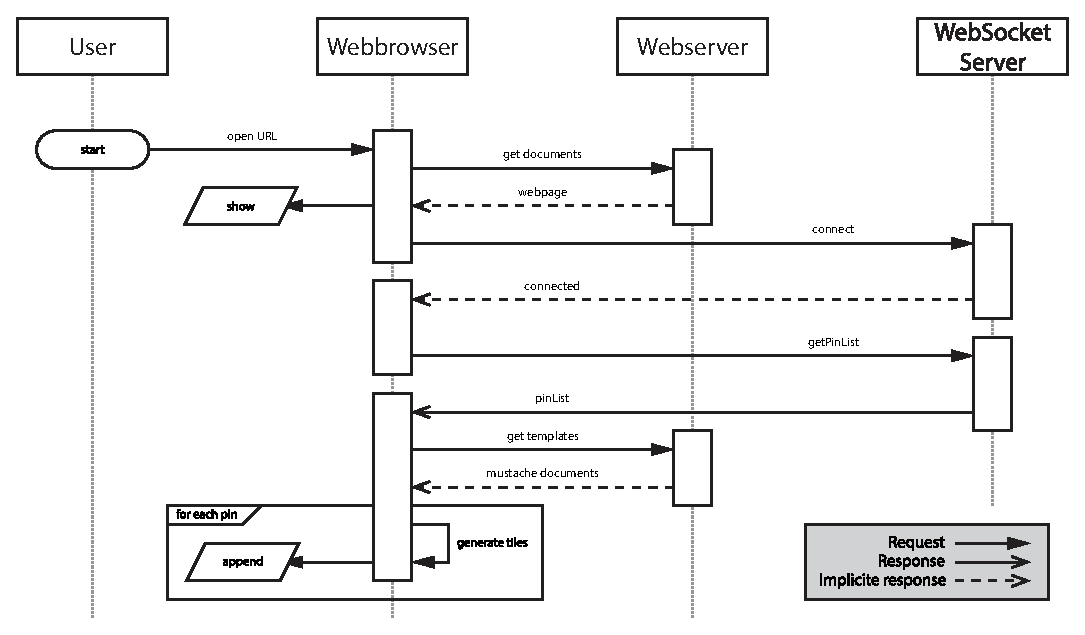
\includegraphics[width = \textwidth]{images/pageload.eps}
\caption{Sequezieller Ablauf bei einem Seitenaufruf}
\label{fig:pageloadSequence}
\end{figure}


\section{Interaktion}
Die Kommunikation mit dem WebSocket Server läuft vollständig asynchron ab. Es wird grundsätzlich keine direkte Antwort auf eine Anfrage erwartet, um bei eventuell schlechter Netzwerverbindung nicht das Interface zu blockieren. Abbildung \ref{fig:interaction} zeigt diesen Vorgang exemplarisch.

\begin{figure}[ht]
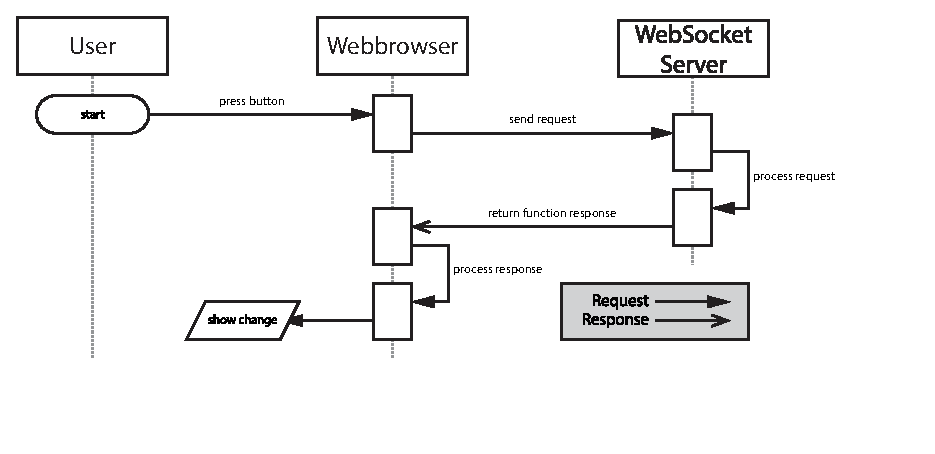
\includegraphics[width = \textwidth]{images/sendRequest.eps}
\caption{Verarbeitung einer User-Interaktion}
\label{fig:interaction}
\end{figure}


\section{WebSocket Server}
Der WebSocket Server ist vollständig in JavaScript/Node.js implementiert und modular aufgebaut. Alle notwendigen Dateien finden sich im Verzeichnes \textit{node/}.\\
Eine Besonderheit von JavaScript/Node.js ist es, dass sich Module grundsätzlich ähnlich wie ein Singleton Pattern verhalten. Dabei wird bei einem erneuten Aufruf von \textit{require()} keine neue Instanz erzeugt, sondern Referenzen auf die Erste übergeben.\\
So müssen bei asynchronen Funktionsaufrufen nicht alle benötigten Variablen übergeben werden und es wird sichergestellt, dass alle Funktionen auf denselben WebSocket zugreifen. Dies ist vor allem wichtig, da Intervalfunktionen, die via \textit{setInterval()} aufgerufen werden, keinen direkten Zugriff erlauben. Zudem sollen laufende Timer bei einem erneuten Besuch der Seite (oder einen reload) ihre Daten direkt wieder an den Browser senden.

\begin{figure}[ht]
\centering
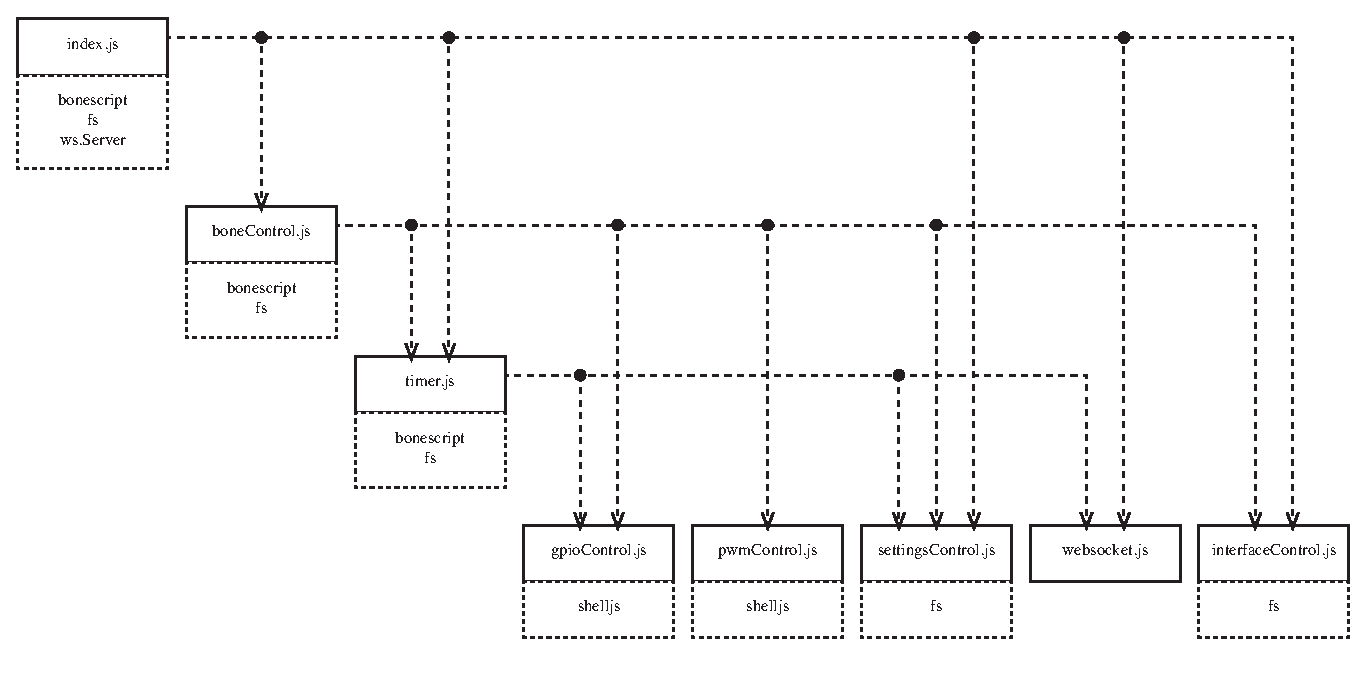
\includegraphics[width = \textwidth]{images/wssDependencies.eps}
\caption{Abhängigkeiten der Module des WebSocket Server}
\label{fig:wssDependencies}
\end{figure}

Abbildung \ref{fig:wssDependencies} zeigt die Abhängigkeit zwischen den einzelnen Modulen. Im Kasten unter dem Modulnamen sind Abhängigkeiten dargestellt, die nicht Teil dieser Implementierung sind.


\subsubsection{index.js}
Die index.js stellt das Hauptdokument dar. Von hier aus wird der Server gestartet. Über den Aufruf \textit{require()} werden die Module des Servers geladen und die Event Listener für die WebSocket Verbindung registriert.

Bei einem erfolgreichen Verbindungsaufbau wird der WebSocket im \textit{websocket}-Objekt referenziert und für alle anderen Module zugänglich gemacht.


\subsection{Models}

\subsubsection{settingsControl.js}
\begin{wrapfigure}[4]{r}{0.25\textwidth}
\vspace{-14pt}
\centering
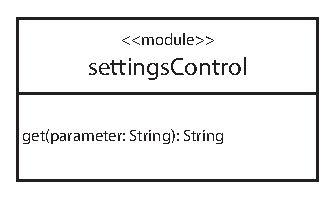
\includegraphics[width = 0.25\textwidth]{images/apiSettingsControl.eps}
\end{wrapfigure}

Das Modul \textit{settingsControl.js} liest die Einstellungsdateien ein und stellt diese programmweit zur Verfügung. Das Modul nutzt dafür die Datei \textit{settings-default.json}, in der alle Basiseinstellungen enthalten sind. Diese Einstellungen werden dann von denen in der Datei \textit{settings.json} überschrieben, sofern das Dokument vorhanden ist. Bei den beiden Dateien handelt es sich um \gls{json}-Dateien nach rfc6455 \cite{rfc6455}.

Es werden nur Parameter überschrieben, die sowohl in den Defaulteinstellungen als auch in den eigenen vorhanden sind. So ist sicherggestellt, dass keine Parameter versehentlich ins System gelangen, die nicht dafür vorgesehen sind. Des Weiteren ist es möglich, nur die Einstellungen einzutragen, die geändert werden sollen.

\subsubsection{interfaceControl.js}
\begin{wrapfigure}[4]{r}{0.25\textwidth}
\vspace{-14pt}
\centering

\includegraphics[width = 0.25\textwidth]{images/apiInterfaceControl.eps}
\end{wrapfigure}

Dieses Modul generiert bei Bedarf eine Liste der verfügbaren Pins und deren Typen sowie deren letztmalige Interfacekonfiguration bezüglich aktiver und inaktiver Kacheln.\\

\noindent Zwei Dateien werden zur Generierung des \textit{interface}-Objekts ausgelesen:

\begin{itemize}
  \item \textit{whitelist.json} enthält eine Liste der Pins mit Informationen über die Verwendbarkeit. Die Liste ist statisch und muss zur Software passen, sie wird vom Programm nicht verändert.
  \item \textit{interface.json} ist eine Stringversion der letzten Interfacekonfiguration. Falls sie existiert, wird ein kombiniertes Objekt generiert um sicherzustellen, dass Informationen über das Interface nicht verloren gehen und eventuell zusätzliche Pins dennoch verfügbar sind.
\end{itemize}

Wenn die WebSocket Verbindung geschlossen wird, wird das im Speicher befindliche Interfaceobjekt in die Datei interface.json geschrieben und kann beim nächsten Aufruf der Seite erneut geladen werden.

\subsubsection{websocket.js}
\begin{wrapfigure}[4]{r}{0.25\textwidth}
\vspace{-14pt}
\centering
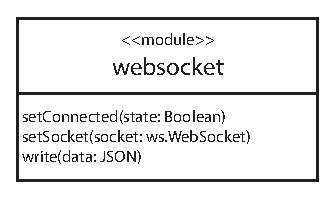
\includegraphics[width = 0.25\textwidth]{images/apiWebsocket.eps}
\end{wrapfigure}

Dieses Modul verwaltet die eigentliche WebSocket Verbindung. Essenziell ist die Funktion \textit{write()}. Hierüber können die restlichen Module direkt auf den WebSocket schreiben. Dabei wird intern geprüft, ob der WebSocket noch offen ist. Wenn eine neue Verbindung hergestellt wurde, wird diese sofort wieder beschrieben.


\subsection{Controllermodule}
Ein weiterer Teil des WebSocket Servers besteht aus einer Reihe von Controllermodulen, die verschiedene Steuerungen übernehmen.

\subsubsection{boneControl.js}
\begin{wrapfigure}[4]{r}{0.25\textwidth}
\vspace{-14pt}
\centering
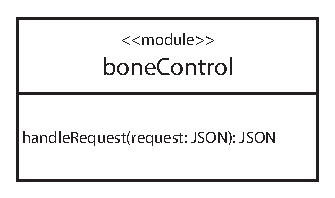
\includegraphics[width = 0.25\textwidth]{images/apiBoneControl.eps}
\end{wrapfigure}

Dieses Modul stellt den Kern der Hardwareansteuerung dar. Eingehende WebSocket Requests werden hier über \textit{type} identifiziert und abgearbeitet. Hierbei wird über eine Switch-Case-Anweisung entschieden, was zu tun ist. Requests mit unbekanntem Typ werden mit einer Fehlermeldung im \textit{response}-Objekt an das Interface zurückgesendet (Abb. \ref{fig:wssResponseHandler}). Die API der Bonescript Bibliothek ist in dieser Liste weitgehend abgebildet. Daneben werden hier auch sämtliche Parameter für das Interface zusammengestellt und an den Browser gesendet.

\begin{figure}[ht]
\centering
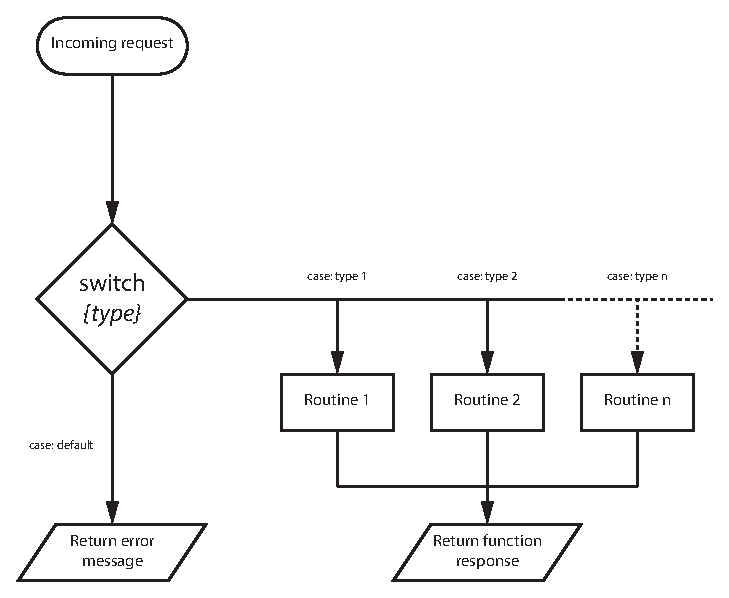
\includegraphics[width = 0.5\textwidth]{images/wssResponseHandler.eps}
\caption{Schematische Arbeitsweise des Response Handlers}
\label{fig:wssResponseHandler}
\end{figure}


\subsubsection{timer.js}

\begin{wrapfigure}[4]{r}{0.25\textwidth}
\vspace{-14pt}
\centering
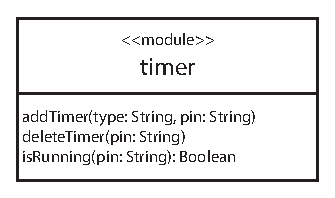
\includegraphics[width = 0.25\textwidth]{images/apiTimer.eps}
\end{wrapfigure}

Mit Hilfe dieses Moduls werden digitale und analoge Inputs verwaltet. Über eine Switch-Case-Anweisung wird geprüft, ob es sich um einen analogen oder digitalen Input handelt und dann mit Hilfe von \textit{setInterval()} ein Timer gestartet, der zyklisch eine anonyme Callbackfunktion aufruft. Das zeitliche Interval wird dem Settingsmodul entnommen. Die Funktionen senden die Ergebnisse selbstständig an die Webseite. Fehlende Dateien, Links oder Ordner werden ebenfalls automatisch erstellt. Um den Timer wieder beenden zu können, wird die Funktion zusätzlich in einem lokalen \textit{Timer}-Objekt registriert.

\paragraph{Digital Input} Um unnötiges Datenvolumen zu vermeiden prüft diese Funktion zunächst, ob sich der Pinstatus gegenüber der letzten Abfrage geändert hat. Nur wenn sich der Wert unterscheidet, wird er an das Interface gesendet (Abb. \ref{fig:wssTimerDigital}).

\begin{figure}[ht]
\centering
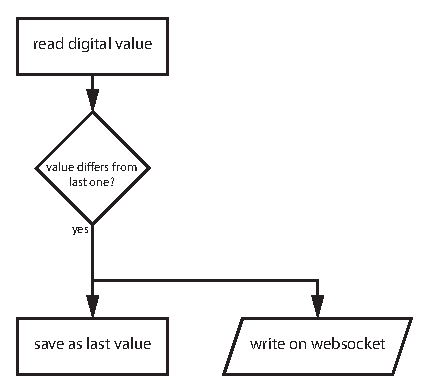
\includegraphics[width = 0.5\textwidth]{images/wssTimerDigital.eps}
\caption{Anonyme \textit{digitalRead}-Funktion}
\label{fig:wssTimerDigital}
\end{figure}

\paragraph{Analog Input} Die Funktion für den analogen Input produziert einen kontinuierlichen Datenstrom, um ein fließendes Diagramm auf der Webseite zu realisieren und speichert diese Daten parallel in einer standardkonformen CSV-Datei \cite{rfc4180} (Abb. \ref{fig:wssTimerAnalog}).

\begin{figure}[ht]
\centering
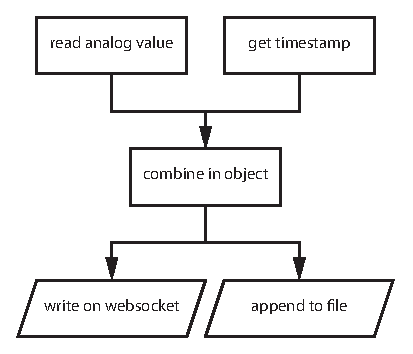
\includegraphics[width = 0.5\textwidth]{images/wssTimerAnalog.eps}
\caption{Anonyme \textit{analogRead}-Funktion}
\label{fig:wssTimerAnalog}
\end{figure}

\subsection{Bypassmodule}
Die Bonescript Bibliothek weist in einigen Fällen Fehler oder fehlende Features auf. Intern arbeitet die Bibliothek mit \gls{devicetree} Overlays, wobei es nicht möglich ist diese wieder zu entladen. Dies ist vor allem wichtig, wenn \gls{pwm}-Ausgänge blockiert wurden, um einen zweiten synchronen Ausgang zu erhalten. Um diese Funktionalität zu implementieren, wurden zwei Bypassmodule geschrieben, die das digital I/O- und das PWM-Management übernehmen.

\subsubsection{gpioControl.js}
\begin{wrapfigure}[4]{r}{0.25\textwidth}
\vspace{-14pt}
\centering
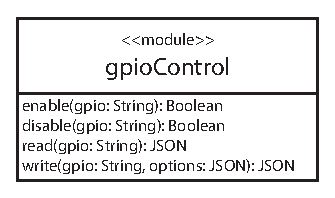
\includegraphics[width = 0.25\textwidth]{images/apiGPIOControl.eps}
\end{wrapfigure}

Dieses Modul steuert die digitalen I/O direkt über das Dateisystem. Dazu werden die in der Bonescript Bibliothek hinterlegten Pin IDs genutzt.\\

Das Modul stellt Funktionen zum Aktivieren und Deaktivieren der \gls{gpio} zur Verfügung sowie zum Lesen und Schreiben der Parameter. Parameter werden in Form eines \gls{json}-Objektes übergeben und sind jeweils optional.

\subsubsection{pwmControl.js}
\begin{wrapfigure}[4]{r}{0.25\textwidth}
\vspace{-14pt}
\centering
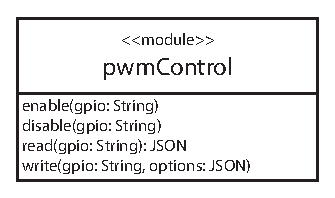
\includegraphics[width = 0.25\textwidth]{images/apiPWMControl.eps}
\end{wrapfigure}

Die API dieses Moduls verhält sich analog zu dem der \gls{gpio}. Intern werden die Device Tree Overlays der Bonescript Bibliothek verwendet. Diese werden per Filesystem über den \gls{capemgr} geladen.

\section{Webseite} Bei der Implementierung steht die Funktionalität im Fokus. Daher wurde so viel wie möglich mit bereits existierenden Bibliotheken gearbeitet, um Design und Darstellung umzusetzen. Diese Bibliotheken basieren intern auf \gls{html}, \gls{css} und \gls{js}.\\
Die Webseite selbst besteht daher nur aus einem einzigen \gls{html}-Dokument, in dem die Basisstruktur der Seite definiert wird. In der index.html werden auch alle globalen Objekte wie die WebSocket Verbindung und die Pinliste angelegt.\\

Bei einem Seitenaufruf werden zunächst die benötigten Bibliotheken beim Webserver angefordert und geladen. Das Event \textit{document.ready} stößt dann den Verbindungsaufbau zum WebSocket Server an. Ist die Verbindung hergestellt, wird das Event \textit{websocket.onopen} ausgelöst und die aktuelle Pinkonfiguration vom Server angefordert.

Die weiteren Inhalte werden dynamisch via JavaScript und \gls{html}-Templates generiert.


\subsection{Skriptdokumente}
Die Funktionen für die Webseite sind analog zu den Modulen des WebSocket Servers aufgeteilt. Die Skriptdokumente der Webseite sind jeweils via \gls{json} mit einem Pseudo-Namespace versehen. Funktionen und Objekte sind dabei in einer \gls{json}-Struktur angelegt und können darüber abgerufen werden. Auch Sub-Namespaces sind möglich, um beispielsweise Hilfsfunktionen zu beherbergen (Abb. \ref{lst:pseudeNamespaceJS}).

\begin{figure}[ht]
\begin{lstlisting}
var bonescriptCtrl = {};
    bonescriptCtrl.util = {};
\end{lstlisting}
\caption{Pseudo-Namespace in JavaScript}
\label{lst:pseudeNamespaceJS}
\end{figure}

Da es innerhalb des Browsers keine modulare Struktur wie im WebSocket Server gibt und um daher keinen falschen Eindruck zu erwecken, sind im Folgenden alle Skriptdokumente alphabetisch zusammengestellt.

\begin{longtabu} to \textwidth {
X[1]
X[3]}
\textbf{bonescriptCtrl.js} & Hier werden alle Funktionen zum Absetzen von Steuerbefehlen an den WebSocket Server definiert. Sowohl Befehle für die Hardwaresteuerung als auch für das Interface sind hinterlegt.\newline\\

\textbf{diagramCtrl.js} & Enthält Funktionen, um die Diagramme zu verwalten. Zum einen werden hierüber die Diagramme initialisiert, zum anderen Funktionen zum Hinzufügen neuer Wertepaare und zum Zurücksetzten des Diagramms registriert. Die Zeichengeschwindigkeit ist fest auf 25Hz gesetzt, um die Systemlast möglichst gering zu halten.\newline\\

\textbf{init.js} & Dieses Dokument liefert eine Funktion, \textit{init()}, in der der eigentliche Inhalt der Seite generiert wird. Sobald die Pinliste übermittelt wurde, arbeitet eine For-Each-Schleife jeden einzelnen Pin ab. Dabei werden via synchronem Ajax Request die Templates vom Webserver angefordert. Da die Dokumente zunächst im Cache des Browsers verbleiben, entsteht durch den häufigen Aufruf kein erhöhter Netzwerkverkehr. Im Anschluss werden die Listenerfunktionen an Buttons, etc. angehängt.\newline\\

\textbf{responseHandler.js} & Der Response Handler ist eine Sammlung von Funktionen, um auf eingehende Nachrichten zu reagieren. Zu jedem im WebSocket Server definierten \textit{type} gibt es hier eine entsprechende Funktion. Funktionsnamen sind identisch, damit die Fuktionen direkt aufgerufen werden können.\newline\\

\textbf{util.js} & Dieses Dokument enthält einige Utilityfunktionen, zur einfacheren Bedienung von Bootstrap.\newline\\

\textbf{websocketCtrl.js} & Hier ligen die Listenerfunktionen für die WebSocket Verbindung. Bei einem erfolgreichen Verbindungsaufbau wird der Buttom im Hautfenster verändert und der Initprozess angestoßen. Eingehende Nachrichten werden in \gls{json}-Objekte übersetzt und die entsprechende Funktion aus dem Response Handler aufgerufen.\newline\\
\end{longtabu}


\subsection{Bibliotheken}

\subsubsection{jQuery}
jQuery ist ein \gls{de-facto-standard} zur \gls{dom}-Verwaltung. Diese Bibliothek ermöglicht objektähnliche Verwendung von \gls{html}-Elementen und stellt viele Render- und Animationsfunktionen zur Verfügung.\\

jQuery ist Vorraussetzung für alle weiteren Bibliotheken.


\subsubsection{Bootstrap \& jQuery-UI}
Bootstrap ist für die graphische Darstellung verantwortlich und wird durch einzelne Funktionen aus jQuery-UI ergänzt. Hierbei ermöglicht dieses Framework ein Kachelsystem, das zur Anordnung der Bedienelemente verwendet wird. Dieses System ermöglicht eine dynamische Darstellung, sodass deaktivierte Bedienelemente nicht einfach nur leere Felder hinterlassen. Die aktiven Felder werden vielmehr übersichtlich zusammengerückt. Weiter generiert Bootstrap mit Hilfe von Themes alle Elemente wie Kopfleiste, Buttons oder Eingabemasken.\\


\subsubsection{Flot Diagrams}
Diese Bibliothek dient zum Zeichnen der Diagramme. Im Dokument wird hierfür nur ein Platzhalter eingetragen. Alles weitere ist Aufgabe der Bibliothek. Um neue Messpunkte einzutragen, wird zunächst das Array, welches alle darzustellenden Wertepaare enthält, aktualitisiert und per Funktionsaufruf neu gerendert.


\subsubsection{Mustache.js}
Mustache.js ist eine JavaScript Implementierung des \href{http://mustache.github.io/}{Mustache-Template-Systems}. Mit diesem Werkzeug lassen sich ohne großen Aufwand HTML Templates schreiben, bei denen Variablen in doppelten geschweiften Klammern -- \{\{variable\}\} -- eingesetzt werden. Diese werden in der Laufzeit mittels \textit{Mustache.render()} zu einem gültigen HTML String verarbeitet. Da sich die einzelnen Kacheln nur in der Pinbezeichnung unterscheiden, wurde für jeden der drei Kacheltypen jeweils ein Template entworfen.